% This file is part of the DDD project.
% Copyright 2014 David W. Hogg (NYU).

\documentclass[aspectratio=169]{beamer}

\setbeamertemplate{footline}[text line]{%
  \parbox{\linewidth}{\vspace*{-8pt}~\hfill David W. Hogg~/~\insertpagenumber}}
\setbeamertemplate{navigation symbols}{}

\newcommand{\foreign}[1]{\textsl{#1}}
\newcommand{\etal}{\foreign{et~al}}
\renewcommand{\emph}[1]{\textbf{#1}}
\newcommand{\project}[1]{\textsl{#1}}
\newcommand{\Kepler}{\project{Kepler}}

\begin{document}

\begin{frame}
  \frametitle{David W. Hogg}
  \begin{itemize}
  \item go deep-ish on extra-Solar planets
    \begin{itemize}
    \item high-level (planet populations) to low-level (detector pixels)
    \item there are gains available at every level
    \item probabilistic inference is my primary technology
    \end{itemize}
  \item other astrophysics projects
  \item methods \& tools
  \item \emph{feel free to tweet or blog me}
  \end{itemize}
\end{frame}

\begin{frame}
  \frametitle{Extra-Solar planets: How we find them}
  \begin{itemize}
  \item direct imaging \textit{(ten-ish)}
  \item radial velocity \textit{(hundreds)}
  \item \emph{transit} \textit{(thousands)}
    \begin{itemize}
    \item NASA \Kepler\ Satellite
    \item Earth: \emph{84~ppm} (0.000084) signal for 13~h, once per year
    \end{itemize}
  \item astrometry \textit{(zero, for now, but\ldots)}
  \end{itemize}
\end{frame}

\begin{frame}
  \frametitle{Earth and Jupiter analogs}
  \begin{itemize}
  \item because life!
  \item because Solar-System formation!
  \item in \emph{principle}, \Kepler\ is sensitive enough
    \begin{itemize}
    \item some ``habitable planets'' known
    \item all around stars cooler (and smaller) than the Sun
    \end{itemize}
  \end{itemize}
\end{frame}

\begin{frame}
  \frametitle{Exoplanet populations \small{(Foreman-Mackey \etal)}}
  \begin{itemize}
  \item noisy measurements of a bunch of planets
  \item subject to non-trivial completeness or censoring
  \item how to infer properties of the ``de-noised'' and complete population?
    \begin{itemize}
    \item fully probabilistic inference
    \item fewer assumptions than any other studies
    \item more flexible models
    \item with Dan Foreman-Mackey (NYU)
    \end{itemize}
  \end{itemize}
\end{frame}

\begin{frame}
  \frametitle{Exoplanet populations \small{(Foreman-Mackey \etal)}}
  ~\hfill\includegraphics<1>[width=0.75\textwidth]{pgm.pdf}
  ~\hfill\includegraphics<2>[height=0.85\textheight]{results-results.pdf}
  ~\hfill\includegraphics<3>[height=0.85\textheight]{results-rate.pdf}
\end{frame}

\begin{frame}
  \frametitle{Exoplanet populations}
  \begin{itemize}
  \item What changed?
    \begin{itemize}
    \item Propagated uncertainties properly.
    \item Reduced the expected number of Earth analogs (bad).
    \item Predicted that the existing \Kepler\ data contain $9_{-4}^{+6}$ detectable ``Earths'' (good).
    \item \textit{now to find them\ldots}
    \end{itemize}
  \end{itemize}
\end{frame}

\begin{frame}
  \frametitle{Other astrophysics projects}
  \begin{itemize}
  \item weak gravitational lensing
    \begin{itemize}
    \item \project{The Tractor}
    \end{itemize}
  \item Milky Way formation and dynamics
    \begin{itemize}
    \item \project{Gaia} and \project{APOGEE}
    \item dark matter is the ultimate \emph{latent variable field}
    \end{itemize}
  \item calibration and fundamental astronomy
    \begin{itemize}
    \item \project{Sloan Digital Sky Surveys} (now on v. 4)
    \item 2014 Shaw Prize: Eisenstein: \emph{baryon acoustic feature}
    \end{itemize}
  \item citizen science with amateur astronomers
    \begin{itemize}
    \item \project{Astrometry.net}
    \item \project{Open Source Sky Survey}
    \end{itemize}
  \end{itemize}
\end{frame}

\begin{frame}
  \frametitle{NASA \Kepler\ Satellite}
  \includegraphics<1>[width=0.5\textwidth]{750603main_Ball_Kepler_A8468_275_lg_blog_main_horizontal.jpg}%
  \includegraphics<1>[height=0.85\textheight]{Kepler_FOV_hiRes.jpg}
  \includegraphics<2>[width=0.5\textwidth]{750603main_Ball_Kepler_A8468_275_lg_blog_main_horizontal.jpg}%
  \includegraphics<2>[height=0.85\textheight]{FirstLightLogInvertedPink_wslbld2400.jpg}
\end{frame}

\begin{frame}
  \frametitle{NASA \Kepler\ Satellite}
  \begin{itemize}
  \item stared at one patch of sky for 4.1~yr, exposure every 30~min
  \item $10^5$ measurements per star, $10^5$ stars
  \item optimized for stable photometric measurements
    \begin{itemize}
    \item \emph{10~ppm precision}
    \item but \emph{both the spacecraft and stars vary}!
    \end{itemize}
  \end{itemize}
\end{frame}

\begin{frame}
  \frametitle{Flexible models and marginalization \small{(Foreman-Mackey \etal)}}
  ~\hfill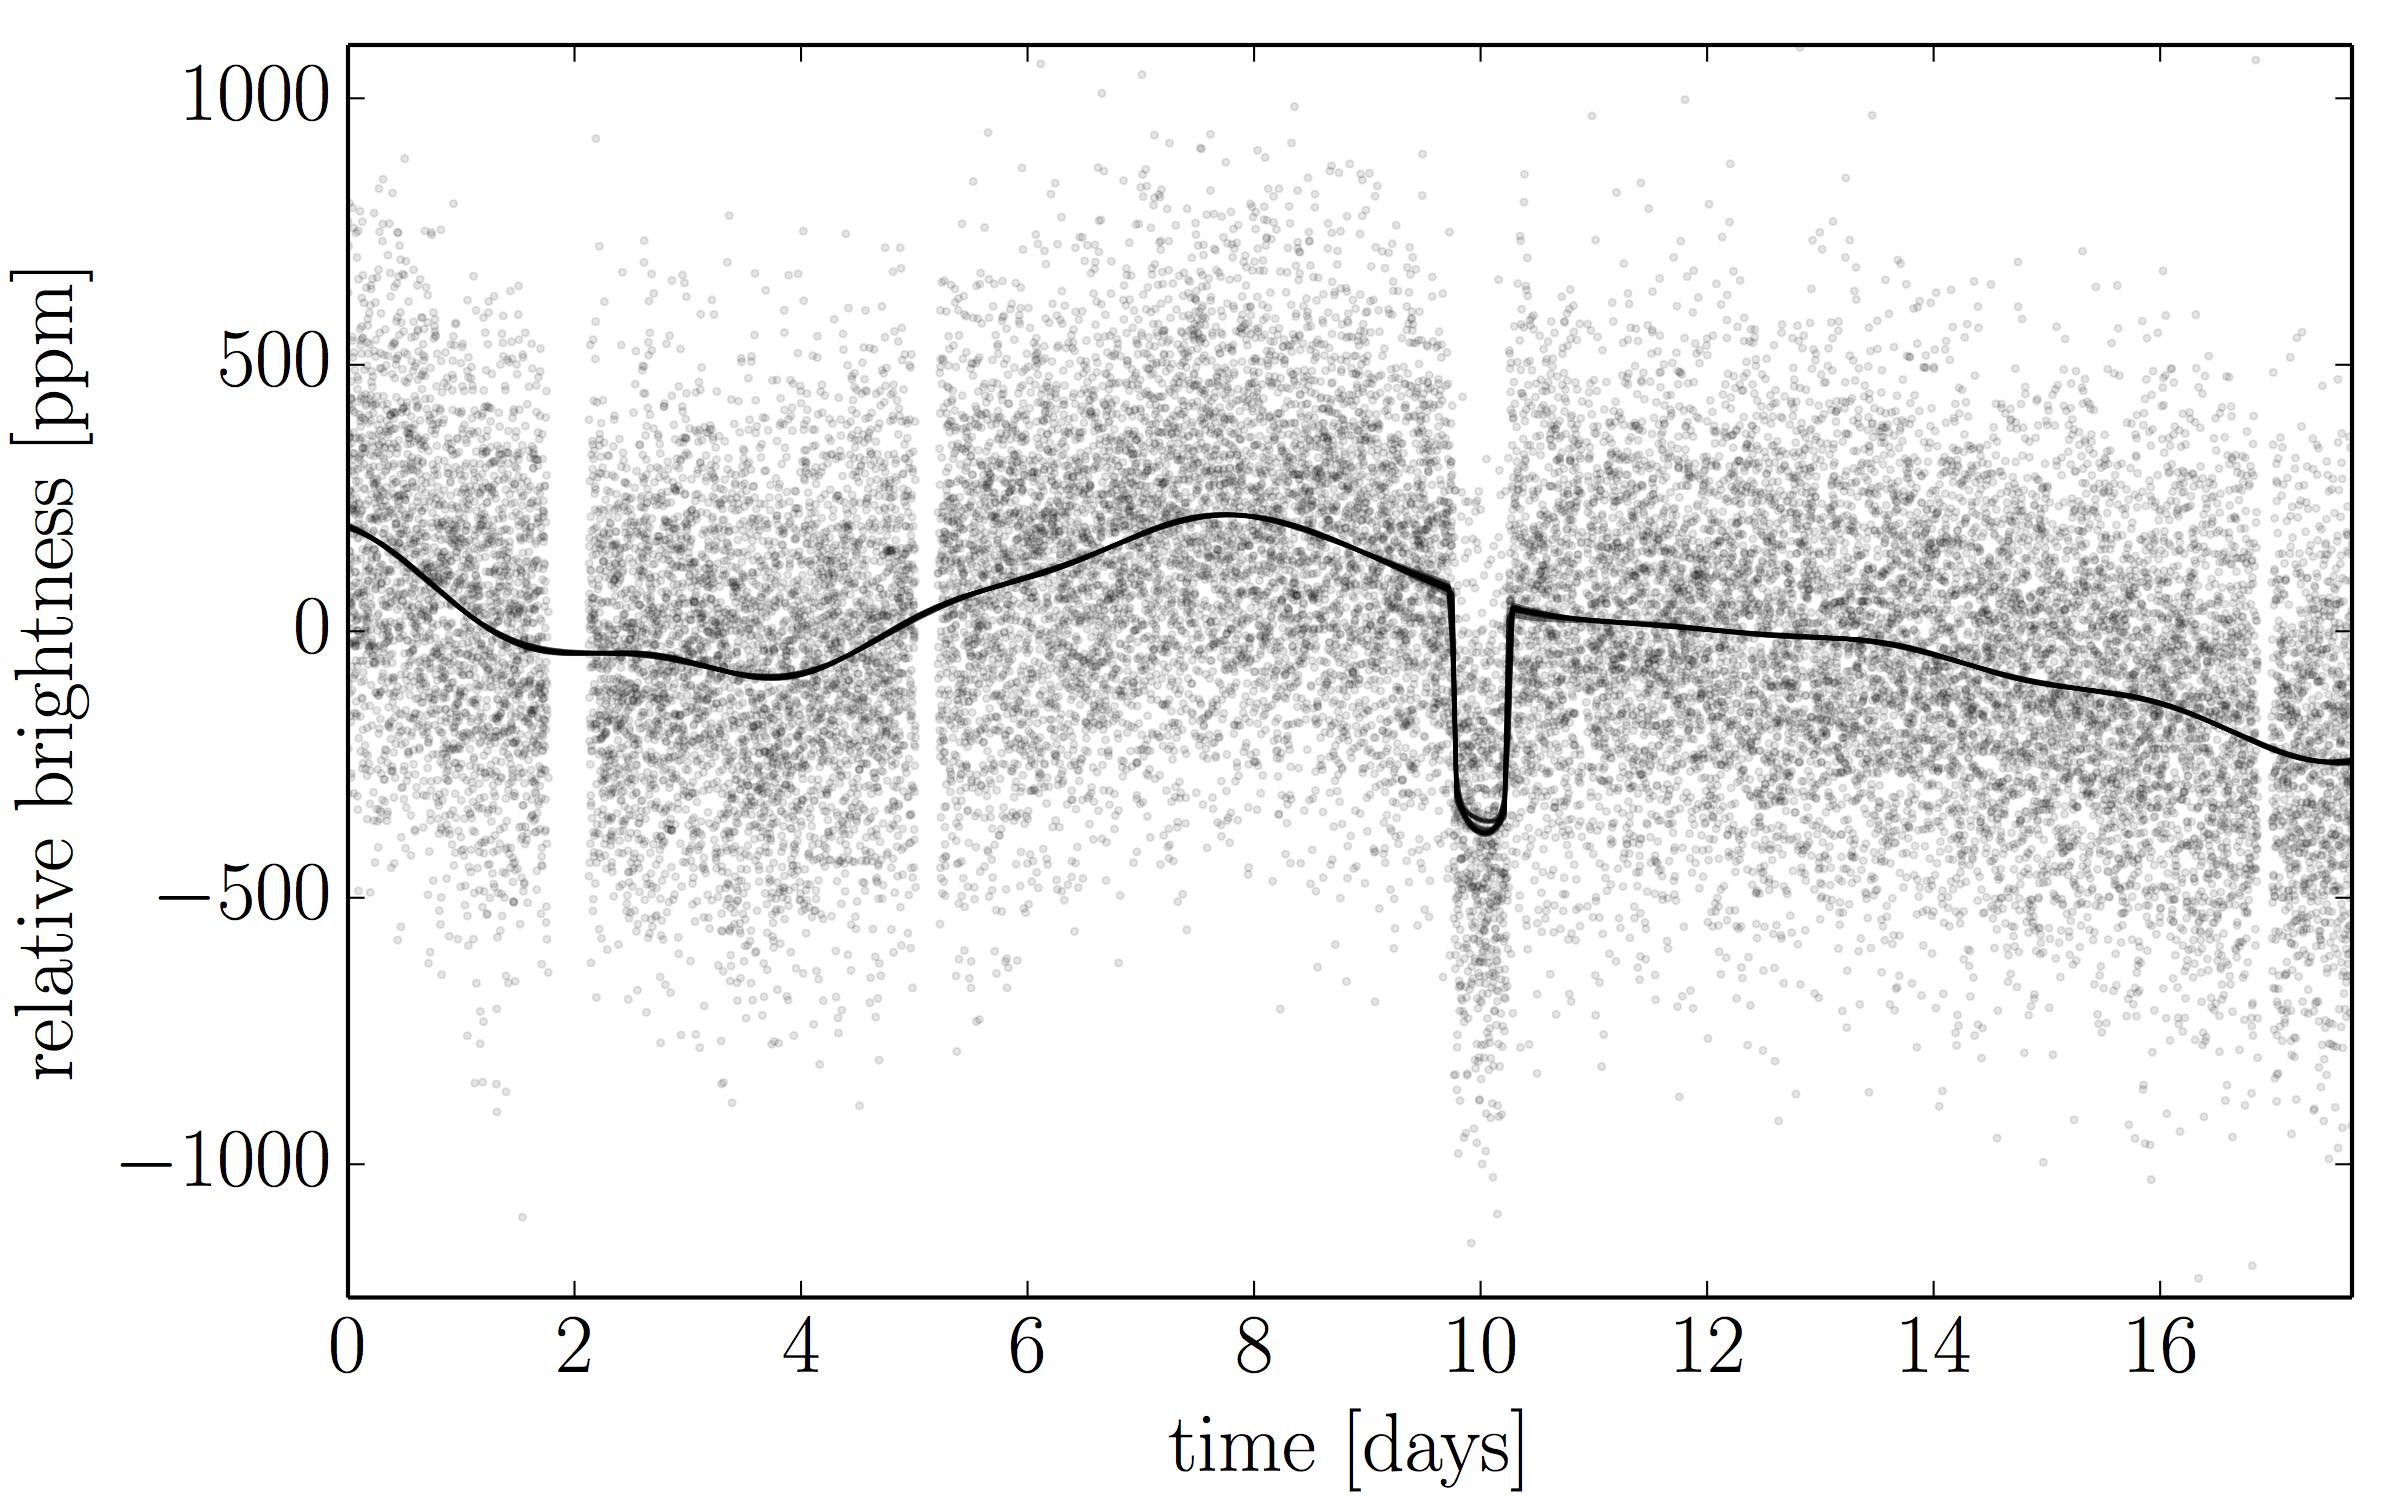
\includegraphics[height=0.85\textheight]{kepler-prediction.png}
\end{frame}

\begin{frame}
  \frametitle{Flexible models and marginalization \small{(Barclay \etal)}}
  ~\hfill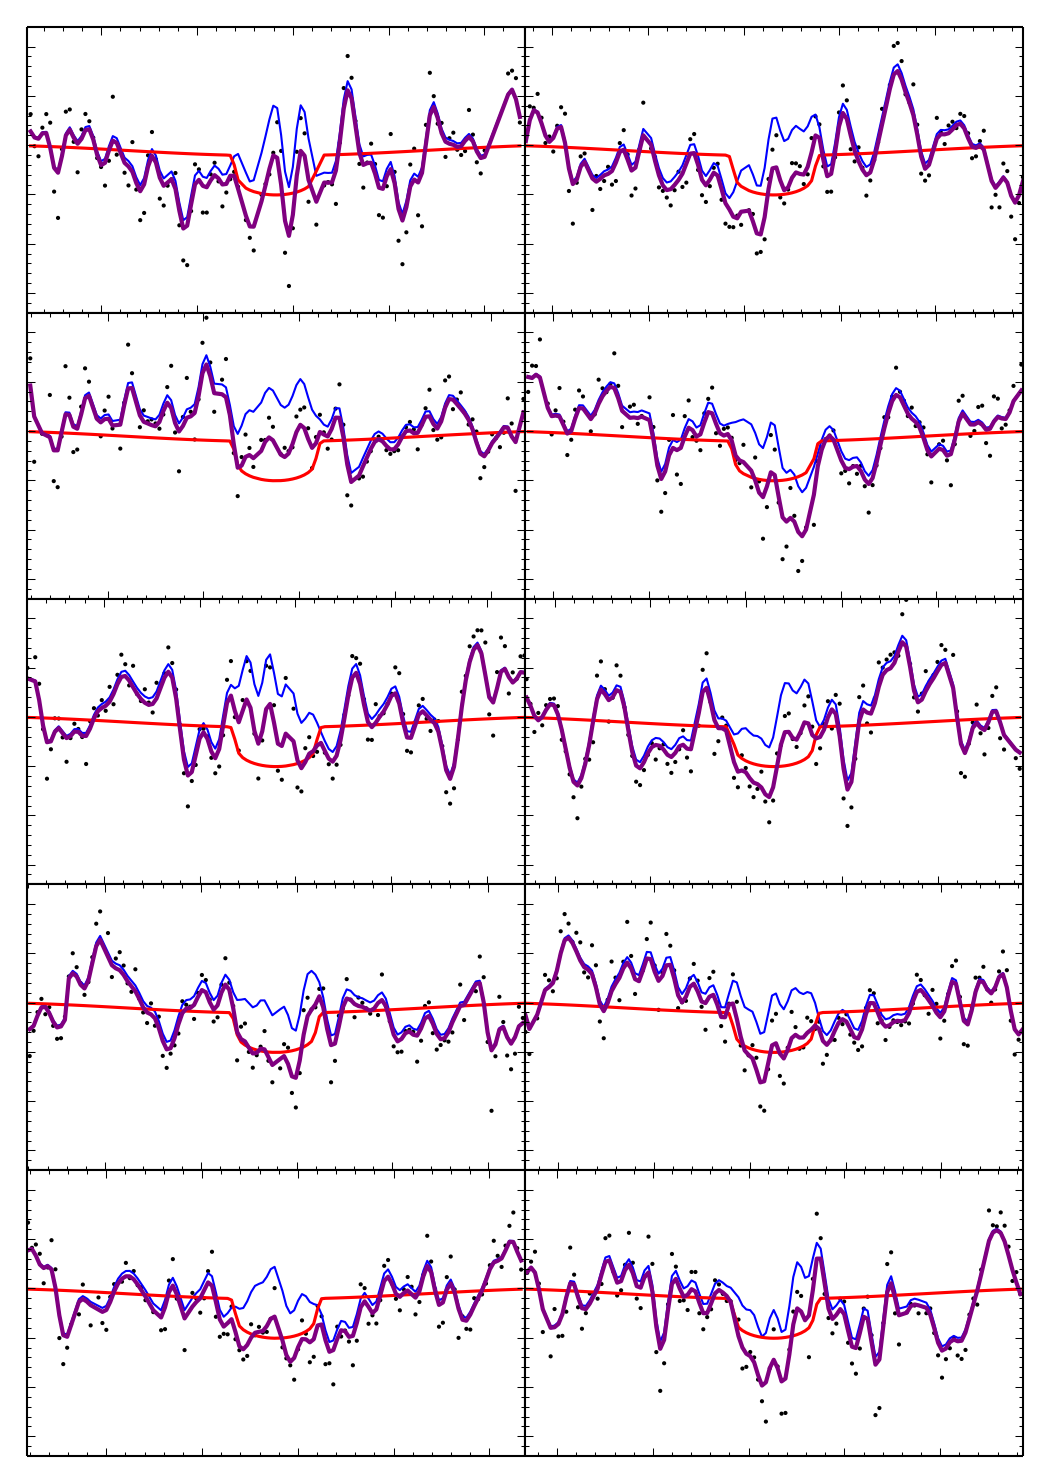
\includegraphics[height=0.85\textheight]{ten_transits.png}
\end{frame}

\begin{frame}
  \frametitle<1>{Methods projects}
  \begin{itemize}
  \item \emph{World's fastest} linear algebra ($n\,\log^2n$) for Gaussian Processes
    \begin{itemize}
    \item capitalizing on hierarchical off-diagonal low-rank (HODLR) form
    \item with Sivaram Ambikasaran (NYU Mathematics)
    \item with Mike O'Neil (NYU Mathematics)
    \end{itemize}
  \item causal inference and astrophysics
    \begin{itemize}
    \item with Jennifer Hill (NYU PRIISM)
    \item with Bernhard Sch\"olkpf (T\"ubingen MPI-IS)
    \end{itemize}
  \item hierarchical modeling with importance sampling
  \item new MCMC methodologies
    \begin{itemize}
    \item ensemble methods that don't require problem-specific tuning
    \item \project{emcee} (top-10-cited astrophysics paper from 2013)
    \item \emph{top-cited methods paper in all of astrophysics} in 2013
    \item with Jonathan Goodman (NYU Mathematics)
    \end{itemize}
  \end{itemize}
\end{frame}

\begin{frame}
  \frametitle{Data-driven self-calibration \small{(Wang \etal)}}
  ~\hfill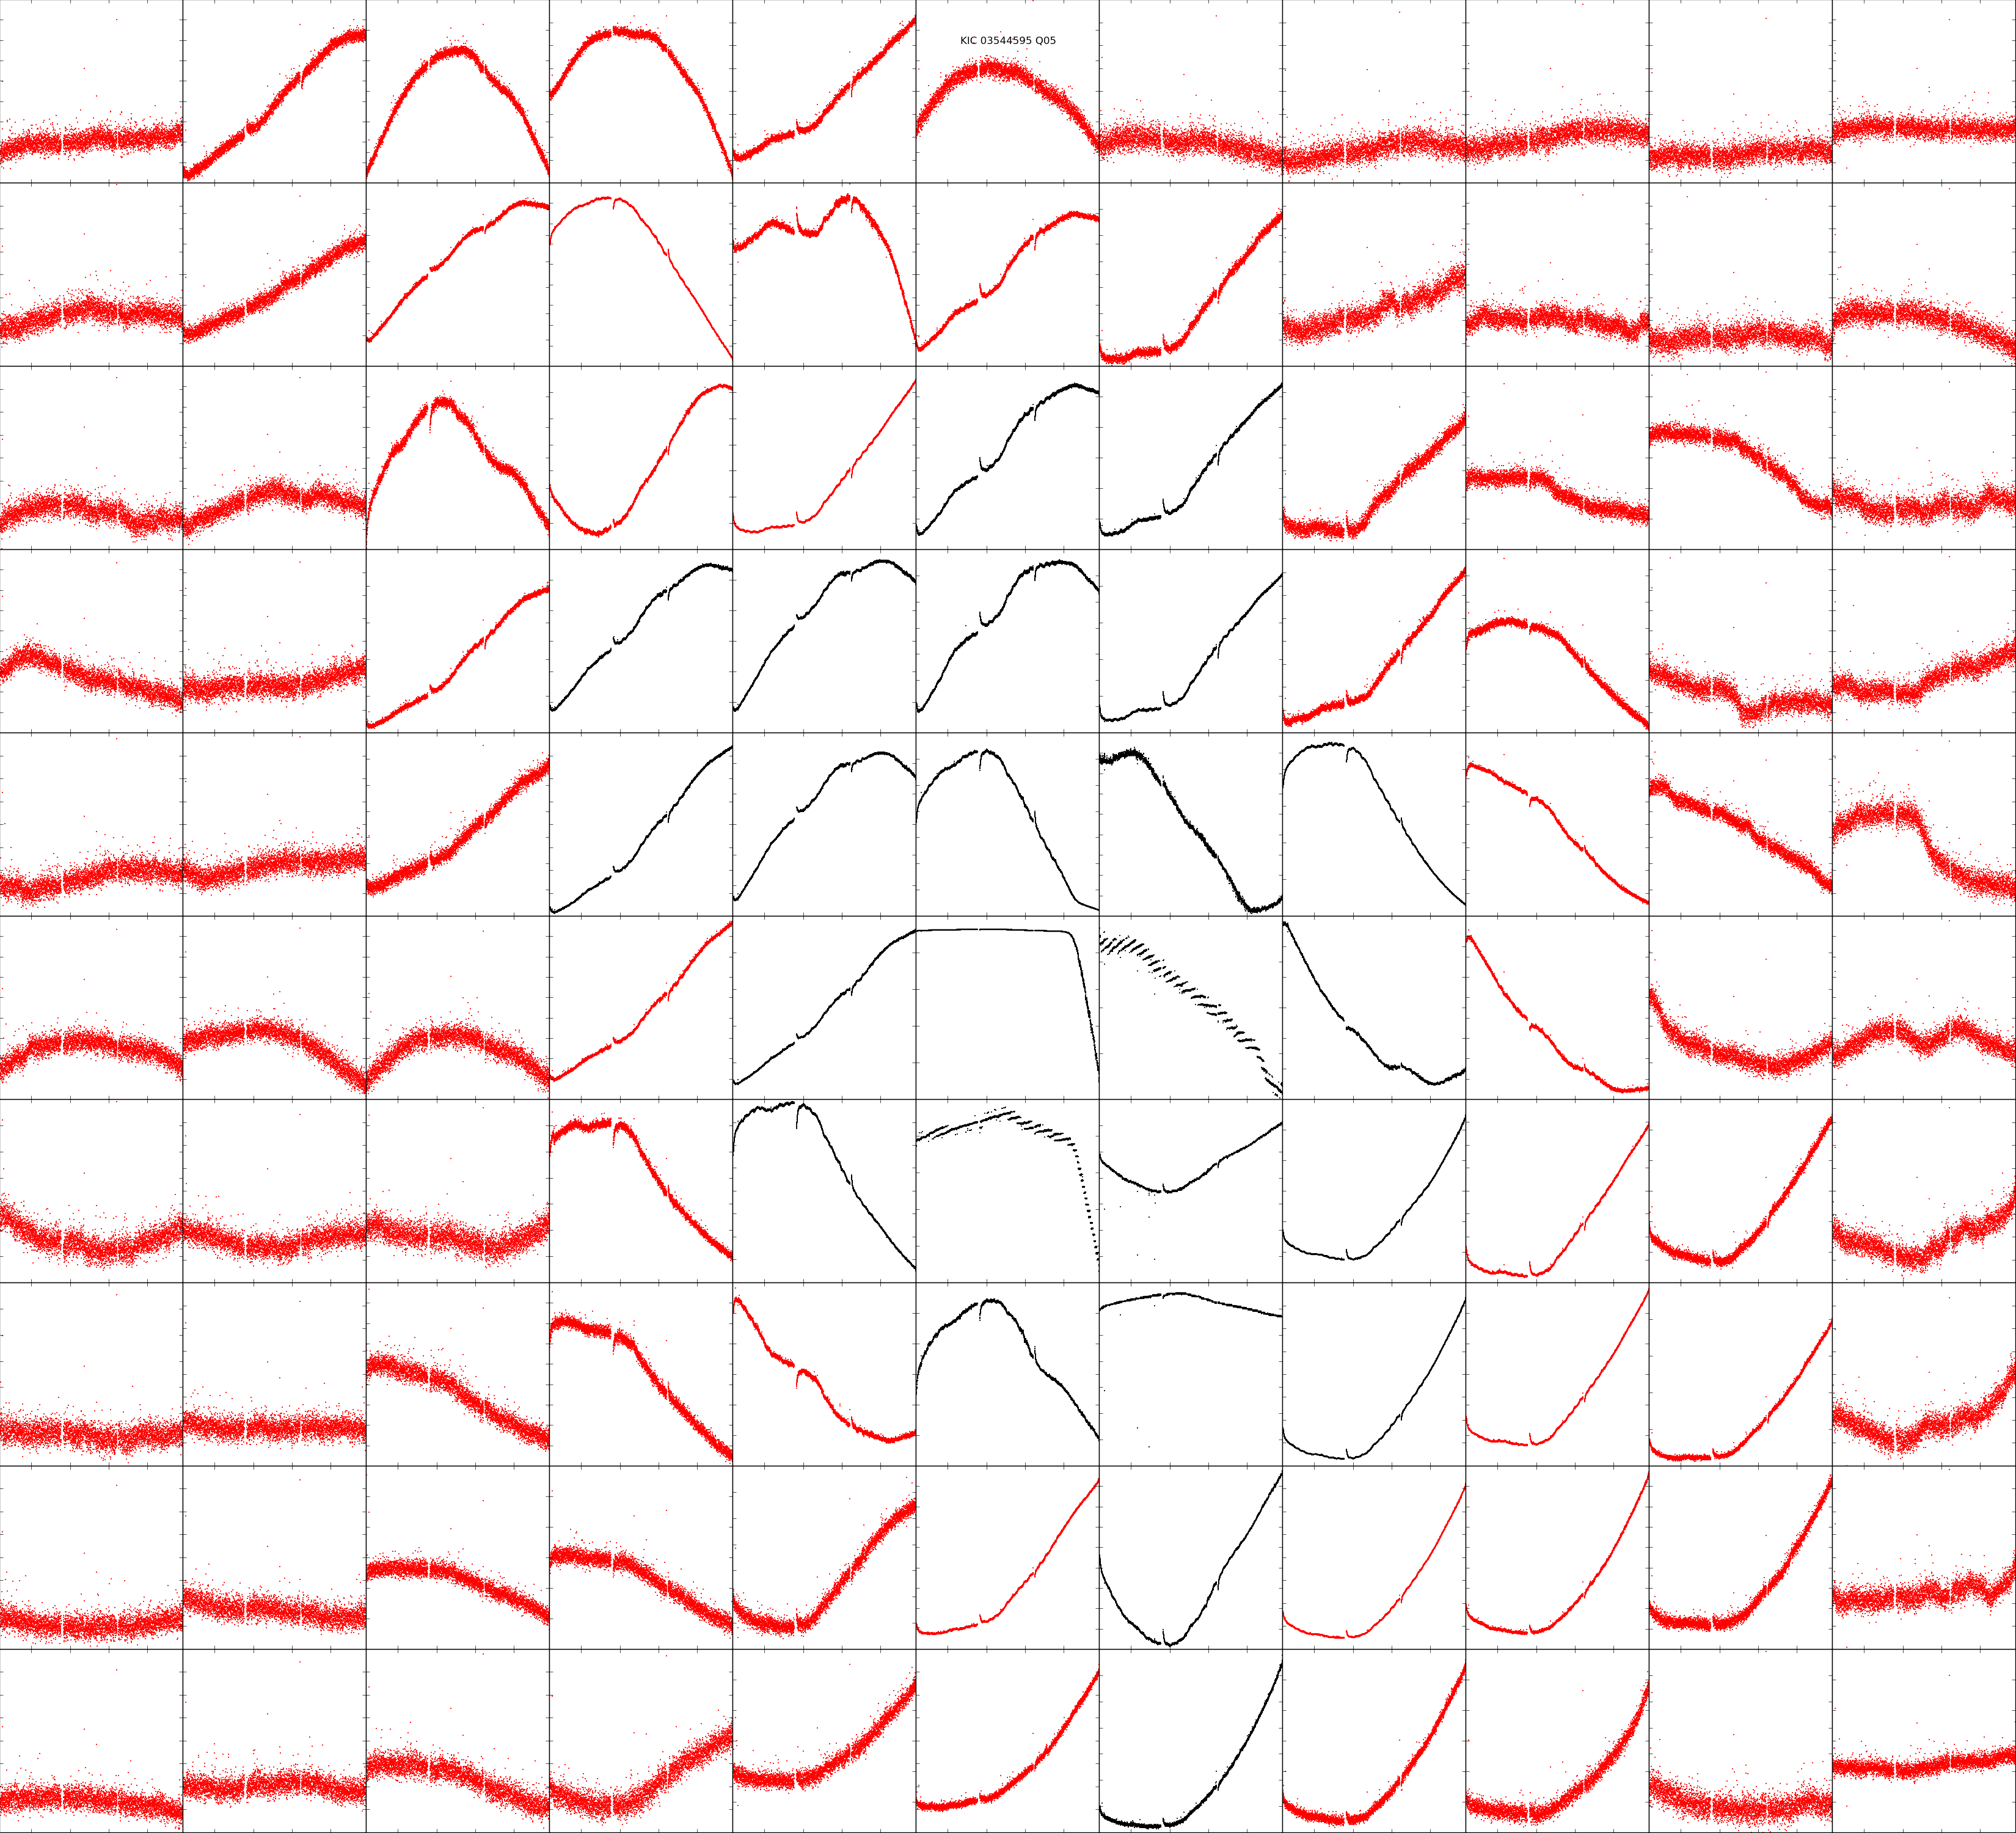
\includegraphics[height=0.85\textheight]{kic_03544595_05_pixels.png}
\end{frame}

\begin{frame}
  \frametitle{Data-driven self-calibration \small{(Wang \etal)}}
  \begin{itemize}
  \item \Kepler\ pixel responses vary with time at the percent level
  \item capitalize on \emph{causal structure} of the problem
    \begin{itemize}
    \item variations widely separated pixels have \emph{in common} must be induced by spacecraft variability
    \end{itemize}
  \item massive regression
    \begin{itemize}
    \item using pixels to fit pixels
    \end{itemize}
  \item train-and-test framework
    \begin{itemize}
    \item controlling model complexity
    \item with Dun~Wang (NYU), Dan~Foreman-Mackey (NYU), Bernhard~Sch\"olkopf (T\"ubingen MPI-IS)
    \item (related to Rafael Irizarry's work)
    \end{itemize}
  \end{itemize}
\end{frame}

\begin{frame}
  \frametitle{Data-driven self-calibration \small{(Wang \etal)}}
  ~\hfill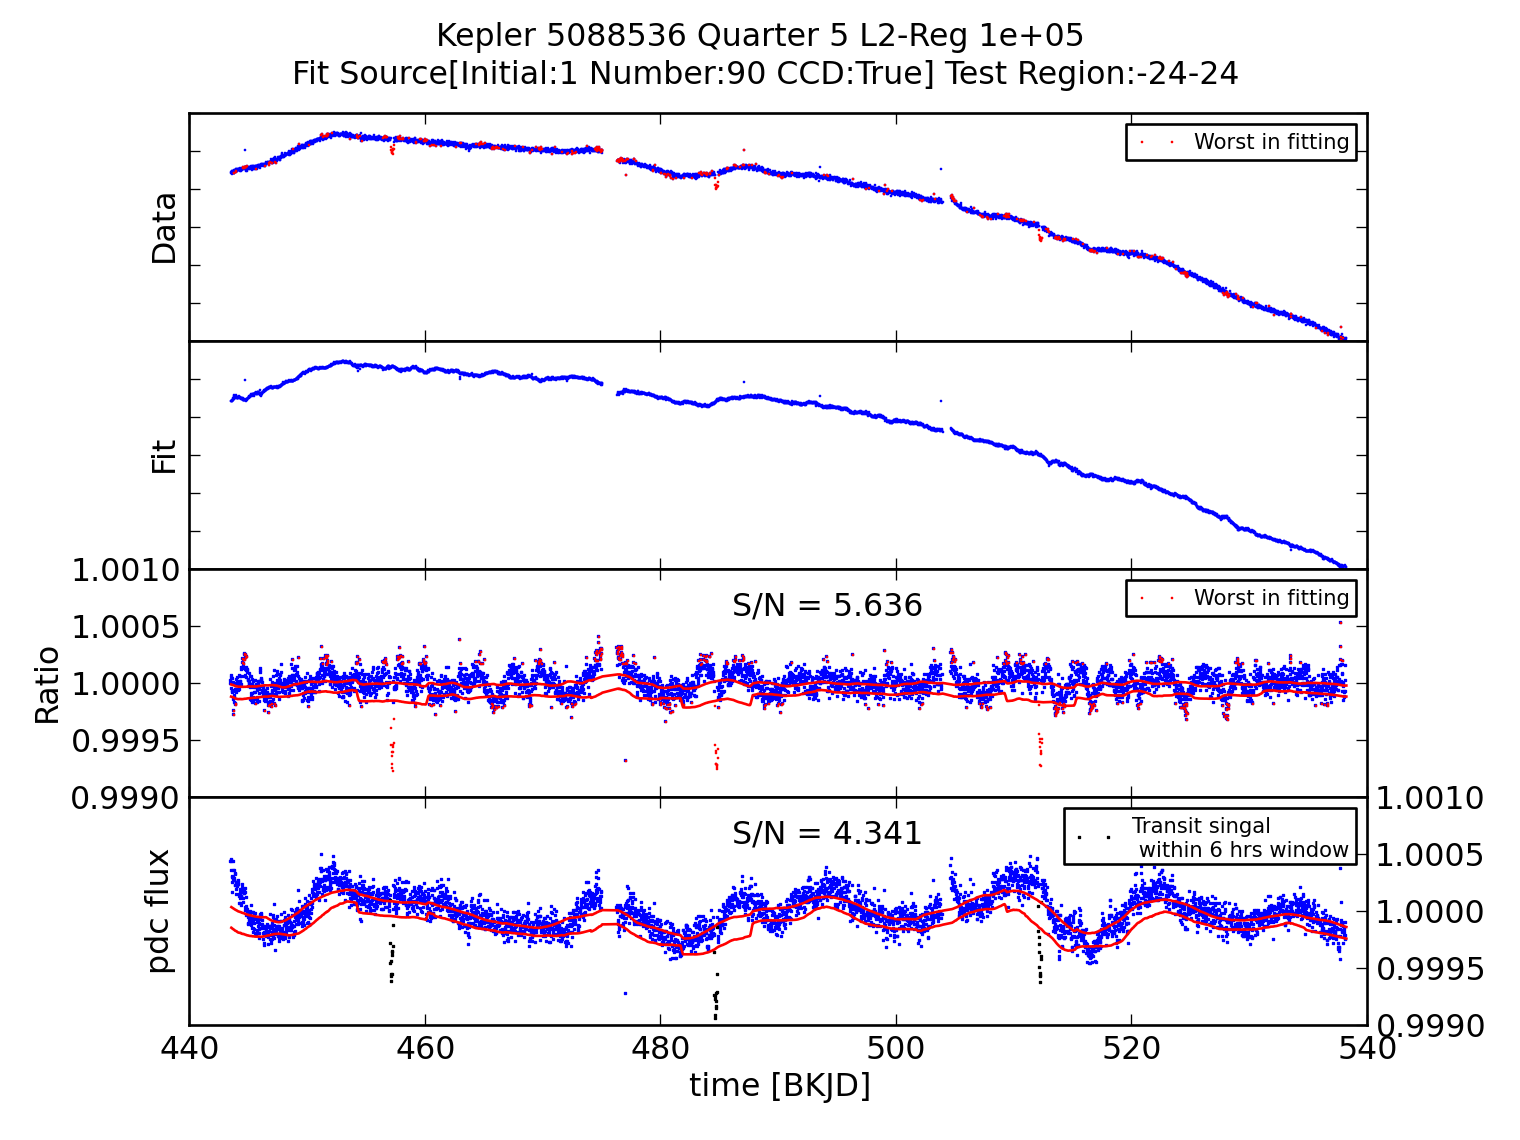
\includegraphics[height=0.85\textheight]{lightCurve_5088536_1_90_q5_reg1e+05_pdc_outlier.png}
\end{frame}

\begin{frame}
  \frametitle{Data-driven self-calibration}
  \begin{itemize}
  \item What will change?
    \begin{itemize}
    \item Will improve signal-to-noise on all transits.
    \item Will deliver interpretable feedback on s/c hardware.
    \end{itemize}
  \item We believe we can make it possible to \emph{detect Earth analogs}.
  \end{itemize}
\end{frame}

\begin{frame}
  \frametitle{Open Science}
  \begin{itemize}
  \item my group runs \emph{wide open}
    \begin{itemize}
    \item open svn, github, blogging
    \item this talk is at \url{https://github.com/davidwhogg/DDD}
    \end{itemize}
  \item \textit{not going to talk about it, but ask me!}
  \end{itemize}
\end{frame}

\begin{frame}
  \frametitle{My role in astrophysics}
  \begin{itemize}
  \item Past
    \begin{itemize}
    \item calibration of \project{SDSS}
    \item fundamental astronomy and measurements
    \item machine learning in astronomy (image recognition)
    \item cosmology with galaxies (baryon acoustic feature)
    \end{itemize}
  \item Present
    \begin{itemize}
    \item methods for probabilistic inference
    \item MCMC sampling methods and code
    \item hierarchical inference
    \item openness
    \end{itemize}
  \item Future
    \begin{itemize}
    \item non-parametrics, Gaussian Processes
    \item flexible instrument models
    \item uncertainty propagation at the catalog level
    \item discovery of the first true Earth analog?
    \end{itemize}
  \end{itemize}
\end{frame}

\end{document}
